\section{Motivation and Challenges}

\subsection{Context} 

\acrfull{das} is a rather new technology that allows for real-time analysis over fiber-optical cables. This technology has gained more recognition within the last decade, and due to their high sensitivity, \acrshort{das} systems can detect subtle environmental changes and anomalies. Analyzing these irregularities is a common and crucial task in various fields, and it can be applied to tasks spanning landslide and earthquake detection as well as railroad and maritime monitoring. The ability to process and interpret \acrshort{das} data effectively is essential for extracting meaningful insights from these complex measurements. \\

\begin{figure}[!h]
    \centering
    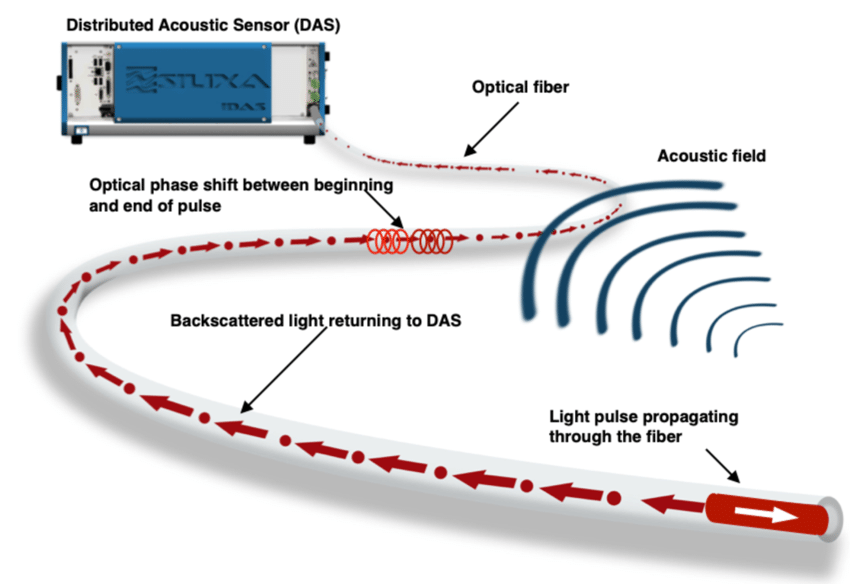
\includegraphics[width=0.7\linewidth]{figures/das.png}
    \caption{Showcase of how \acrshort{das} signals are recorded}
    \label{fig:das-fig}
\end{figure}

Traditionally, clustering-based \acrfull{ml} techniques such as K-MEANS \cite{hartigan1979k} DBSCAN \cite{ester1996density} have been quite popular for anomaly detection \cite{anomaly}. Across the last years, a popular modification to the DBSCAN algorithm, HDBSCAN \cite{rahman2016hdbscandensitybasedclustering}, has also shown prowess in clustering-based anomaly detection \cite{ariyaluran2022clustering}. However, these methods often require manual feature engineering, require labeled datasets, or generally do not scale to large datasets. 

\begin{figure}[!h]
    \centering
    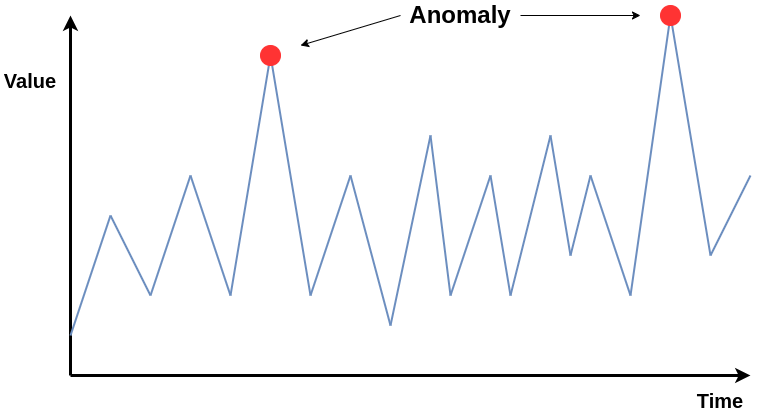
\includegraphics[scale=0.4]{figures/anolay_line.png}
    \caption{Example of anomalies in a time series}
    \label{fig:anomaly_example}
\end{figure}

\acrshort{das} technology in itself has now started garnering attention for research, and several papers have previously studied how one can process this data. \acrshort{ai} and \acrshort{ml} models have been constructed for looking at time series data and analyzing sensor data, although several of these have been studied.  Only recently has \acrshort{ai}


\subsection{Motivating challenges}. 

\acrfull{cgf} spend a lot of time and resources on processing and analyzing \acrshort{das} data. Current tools for processing are quite slow and do not utilize parallelization techniques that have the potential to drastically speed up computations. Additionally, analysis often uses more traditional signal processing techniques, not leveraging the potential benefits of more novel \acrshort{ann} methods. \\ 


Recorded \acrshort{das} data has the potential to become quite large, up to several terabytes per experiment, underlying the importance of efficient algorithm design and processing techniques. Generally, languages such as Python and Matlab are used for DAS analysis due to their framework for data science applications. However, these programming languages are not designed for data-intensive applications without having to leverage languages such as C. Julia is a more novel language aimed at both data science and in general \acrfull{hpc} applications, and could prove really powerful as an alternative to an existent program.


However, with the upcoming of \acrshort{das}, both unsupervised and supervised \acrfull{dl} methods have proven to produce even better results for anomaly detection. For \acrshort{das} data specifically, both scalability and manual labeling can become quite tedious or outright non-feasible. For 

In later years, unsupervised learning has returned after the explosion of generative models [CITE]. Compared to their supervised alternatives, unsupervised do not require manual labeling. They're, therefore, not prone to some of the more common problems within supervised methods, such as detecting irregular events.   are well suited for detecting novel anomalies \cite{wei2022lstmautoencoder, srivastava2016unsupervised} compared to its supervised alternatives, and do not require manual labeling. This makes them 

Current autoencoder-based approaches to anomaly detection of \acrshort{das} do not emphasize the overall memory consumption or the conversion of models to a real-time environment. This 



Previous work on this data \cite{projthesis} revolved around processing \acrshort{hdf5} files as fast and efficiently as possible, trying to parallelize already existent code, and take advantage of newer technologies, such as Julia.
